\documentclass{article}

\def \lastexercisenumber {0}

% ---------------------------------------------------------------- %
% short package descriptions are copied from
% https://ctan.org/

% ---------------------------------------------------------------- %

% Accept different input encodings
\usepackage[utf8]{inputenc}

% Standard package for selecting font encodings
\usepackage[T1]{fontenc}

% ---------------------------------------------------------------- %

% Multilingual support for Plain TEX or LATEX
\usepackage[ngerman]{babel}

% ---------------------------------------------------------------- %

% Set all page margins to 1.5cm
\usepackage{fullpage}

% Margin adjustment and detection of odd/even pages
\usepackage{changepage}

% Flexible and complete interface to document dimensions
\usepackage{geometry}

% ---------------------------------------------------------------- %
% mathematics

\usepackage{amsmath}  % AMS mathematical facilities for LATEX
\usepackage{amssymb}
\usepackage{amsfonts} % TEX fonts from the American Mathematical Society
\usepackage{amsthm}   % Typesetting theorems (AMS style)

% Mathematical tools to use with amsmath
\usepackage{mathtools}

% Support for using RSFS fonts in maths
\usepackage{mathrsfs}

% Commands to produce dots in math that respect font size
\usepackage{mathdots}

% "Blackboard-style" cm fonts
\usepackage{bbm}

% Typeset in-line fractions in a "nice" way
\usepackage{nicefrac}

% Typeset quotient structures with LATEX
\usepackage{faktor}

% Vector arrows
\usepackage{esvect}

% St Mary Road symbols for theoretical computer science
\usepackage{stmaryrd}

% Three series of mathematical symbols
\usepackage{mathabx}

% ---------------------------------------------------------------- %
% algorithms

% Package for typesetting pseudocode
\usepackage{algpseudocode}

% Typeset source code listings using LATEX
\usepackage{listings}

% Reimplementation of and extensions to LATEX verbatim
\usepackage{verbatim}

% If necessary, please use the following 2 packages locally, but never both.
% This is because the algorithm environment gets defined in both packages, which leads to name conflicts.
% \usepackage{algorithm2e}
% \usepackage{algorithm}

% ---------------------------------------------------------------- %
% utilities

% A generic document command parser
\usepackage{xparse}

% Extended conditional commands
\usepackage{xifthen}

% e-TEX tools for LATEX
\usepackage{etoolbox}

% Define commands with suffixes
\usepackage{suffix}

% Extensive support for hypertext in LATEX
\usepackage{hyperref}

% Driver-independent color extensions for LATEX and pdfLATEX
\usepackage{xcolor}

% ---------------------------------------------------------------- %
% graphics

% -------------------------------- %

\usepackage{tikz}

% MISC
\usetikzlibrary{patterns}
\usetikzlibrary{decorations.markings}
\usetikzlibrary{positioning}
\usetikzlibrary{arrows}
\usetikzlibrary{arrows.meta}
\usetikzlibrary{overlay-beamer-styles}

% finite state machines
\usetikzlibrary{automata}

% turing machines
\usetikzlibrary{calc}
\usetikzlibrary{chains}
\usetikzlibrary{decorations.pathmorphing}

% -------------------------------- %

% Draw tree structures
\usepackage[noeepic]{qtree}

% Enhanced support for graphics
\usepackage{graphicx}

% Figures broken into subfigures
\usepackage{subfig}

% Improved interface for floating objects
\usepackage{float}

% Control float placement
\usepackage{placeins}

% Include PDF documents in LATEX
\usepackage{pdfpages}

% ---------------------------------------------------------------- %

% Control layout of itemize, enumerate, description
\usepackage[inline]{enumitem}

% Intermix single and multiple columns
\usepackage{multicol}
\setlength{\columnsep}{1cm}

% Coloured boxes, for LATEX examples and theorems, etc
\usepackage{tcolorbox}

% ---------------------------------------------------------------- %
% tables

% Tabulars with adjustable-width columns
\usepackage{tabularx}

% Tabular column heads and multilined cells
\usepackage{makecell}

% Publication quality tables in LATEX
\usepackage{booktabs}

% ---------------------------------------------------------------- %
% bibliography and quoting

% Sophisticated Bibliographies in LATEX
\usepackage[backend = biber, style = alphabetic]{biblatex}

% Context sensitive quotation facilities
\usepackage{csquotes}

% ---------------------------------------------------------------- %

% ---------------------------------------------------------------- %
% special letters

\newcommand{\N}{\mathbb N}
\newcommand{\Z}{\mathbb Z}
\newcommand{\Q}{\mathbb Q}
\newcommand{\R}{\mathbb R}
\newcommand{\C}{\mathbb C}
\newcommand{\K}{\mathbb K}
\newcommand{\T}{\mathbb T}
\newcommand{\E}{\mathbb E}
\newcommand{\V}{\mathbb V}
\renewcommand{\S}{\mathbb S}
\renewcommand{\P}{\mathbb P}
\newcommand{\1}{\mathbbm 1}
\newcommand{\G}{\mathbb G}

\newcommand{\iu}{\mathrm i}

% ---------------------------------------------------------------- %
% quantors

\newcommand{\Forall}        {\forall ~}
\newcommand{\Exists}        {\exists ~}
\newcommand{\nExists}       {\nexists ~}
\newcommand{\ExistsOnlyOne} {\exists! ~}
\newcommand{\nExistsOnlyOne}{\nexists! ~}
\newcommand{\ForAlmostAll}  {\forall^\infty ~}

% ---------------------------------------------------------------- %
% graphics boxed

\newcommand
{\includegraphicsboxed}
[2][0.75]
{
    \begin{center}
        \begin{tcolorbox}[standard jigsaw, opacityback = 0]

            \centering
            \includegraphics[width = #1 \textwidth]{#2}

        \end{tcolorbox}
    \end{center}
}

\newcommand
{\includegraphicsunboxed}
[2][0.75]
{
    \begin{center}
        \includegraphics[width = #1 \textwidth]{#2}
    \end{center}
}

\NewDocumentCommand
{\includegraphicsgraphicsboxed}
{ O{0.75} O{0.25} m m}
{
    \begin{center}
        \begin{tcolorbox}[standard jigsaw, opacityback = 0]

            \centering
            \includegraphics[width = #1 \textwidth]{#3} \\
            \vspace{#2 cm}
            \includegraphics[width = #1 \textwidth]{#4}

        \end{tcolorbox}
    \end{center}
}

\NewDocumentCommand
{\includegraphicsgraphicsunboxed}
{ O{0.75} O{0.25} m m}
{
    \begin{center}

        \centering
        \includegraphics[width = #1 \textwidth]{#3} \\
        \vspace{#2 cm}
        \includegraphics[width = #1 \textwidth]{#4}

    \end{center}
}

% ---------------------------------------------------------------- %
% braces

\newcommand{\pbraces}[1]{{\left  ( #1 \right  )}}
\newcommand{\bbraces}[1]{{\left  [ #1 \right  ]}}
\newcommand{\Bbraces}[1]{{\left \{ #1 \right \}}}
\newcommand{\vbraces}[1]{{\left  | #1 \right  |}}
\newcommand{\Vbraces}[1]{{\left \| #1 \right \|}}

\newcommand{\abraces}[1]{{\left \langle #1 \right \rangle}}

\newcommand{\floorbraces}[1]{{\left \lfloor #1 \right \rfloor}}
\newcommand{\ceilbraces} [1]{{\left \lceil  #1 \right \rceil }}

\newcommand{\dbbraces}    [1]{{\llbracket     #1 \rrbracket}}
\newcommand{\dpbraces}    [1]{{\llparenthesis #1 \rrparenthesis}}
\newcommand{\dfloorbraces}[1]{{\llfloor       #1 \rrfloor}}
\newcommand{\dceilbraces} [1]{{\llceil        #1 \rrceil}}

\newcommand{\dabraces}[1]{{\left \langle \left \langle #1 \right \rangle \right \rangle}}

\newcommand{\abs}  [1]{\vbraces{#1}}
\newcommand{\round}[1]{\bbraces{#1}}
\newcommand{\floor}[1]{\floorbraces{#1}}
\newcommand{\ceil} [1]{\ceilbraces{#1}}

% ---------------------------------------------------------------- %

% MISC

% metric spaces
\newcommand{\norm}[2][]{\Vbraces{#2}_{#1}}
\DeclareMathOperator{\metric}{d}
\DeclareMathOperator{\dist}  {dist}
\DeclareMathOperator{\diam}  {diam}

% O-notation
\newcommand{\landau}{{\scriptstyle \mathcal{O}}}
\newcommand{\Landau}{\mathcal{O}}

% ---------------------------------------------------------------- %

% math operators

% hyperbolic trigonometric function inverses
\DeclareMathOperator{\areasinh}{areasinh}
\DeclareMathOperator{\areacosh}{areacosh}
\DeclareMathOperator{\areatanh}{areatanh}

% special functions
\DeclareMathOperator{\id} {id}
\DeclareMathOperator{\sgn}{sgn}
\DeclareMathOperator{\Inv}{Inv}
\DeclareMathOperator{\erf}{erf}
\DeclareMathOperator{\pv} {pv}

% exponential function as power
\WithSuffix \newcommand \exp* [1]{\mathrm{e}^{#1}}

% operations on sets
\DeclareMathOperator{\meas}{meas}
\DeclareMathOperator{\card}{card}
\DeclareMathOperator{\Span}{span}
\DeclareMathOperator{\conv}{conv}
\DeclareMathOperator{\cof}{cof}
\DeclareMathOperator{\mean}{mean}
\DeclareMathOperator{\avg}{avg}
\DeclareMathOperator*{\argmax}{argmax}
\DeclareMathOperator*{\argsmax}{argsmax}

% number theory stuff
\DeclareMathOperator{\ggT}{ggT}
\DeclareMathOperator{\kgV}{kgV}
\DeclareMathOperator{\modulo}{mod}

% polynomial stuff
\DeclareMathOperator{\ord}{ord}
\DeclareMathOperator{\grad}{grad}

% function properties
\DeclareMathOperator{\ran}{ran}
\DeclareMathOperator{\supp}{supp}
\DeclareMathOperator{\graph}{graph}
\DeclareMathOperator{\dom}{dom}
\DeclareMathOperator{\Def}{def}
\DeclareMathOperator{\rg}{rg}

% matrix stuff
\DeclareMathOperator{\GL}{GL}
\DeclareMathOperator{\SL}{SL}
\DeclareMathOperator{\U}{U}
\DeclareMathOperator{\SU}{SU}
\DeclareMathOperator{\PSU}{PSU}
% \DeclareMathOperator{\O}{O}
% \DeclareMathOperator{\PO}{PO}
% \DeclareMathOperator{\PSO}{PSO}
\DeclareMathOperator{\diag}{diag}

% algebra stuff
\DeclareMathOperator{\At}{At}
\DeclareMathOperator{\Ob}{Ob}
\DeclareMathOperator{\Hom}{Hom}
\DeclareMathOperator{\End}{End}
\DeclareMathOperator{\Aut}{Aut}
\DeclareMathOperator{\Lin}{L}

% other function classes
\DeclareMathOperator{\Lip}{Lip}
\DeclareMathOperator{\Mod}{Mod}
\DeclareMathOperator{\Dil}{Dil}

% constants
\DeclareMathOperator{\NIL}{NIL}
\DeclareMathOperator{\eps}{eps}

% ---------------------------------------------------------------- %
% doubble & tripple powers

\newcommand
{\primeprime}
{{\prime \prime}}

\newcommand
{\primeprimeprime}
{{\prime \prime \prime}}

\newcommand
{\astast}
{{\ast \ast}}

\newcommand
{\astastast}
{{\ast \ast \ast}}

% ---------------------------------------------------------------- %
% derivatives

\NewDocumentCommand
{\derivative}
{ O{} O{} m m}
{
    \frac
    {\mathrm d^{#2} {#1}}
    {\mathrm d {#3}^{#2}}
}

\NewDocumentCommand
{\pderivative}
{ O{} O{} m m}
{
    \frac
    {\partial^{#2} {#1}}
    {\partial {#3}^{#2}}
}

\DeclareMathOperator{\Div}{div}
\DeclareMathOperator{\rot}{rot}

% ---------------------------------------------------------------- %
% integrals

\NewDocumentCommand
{\Int}
{ O{} O{} m m}
{\int_{#1}^{#2} #3 ~ \mathrm d #4}

\NewDocumentCommand
{\Iint}
{ O{} O{} m m m}
{\iint_{#1}^{#2} #3 ~ \mathrm d #4 ~ \mathrm d #5}

\NewDocumentCommand
{\Iiint}
{ O{} O{} m m m m}
{\iiint_{#1}^{#2} #3 ~ \mathrm d #4 ~ \mathrm d #5 ~ \mathrm d #6}

\NewDocumentCommand
{\Iiiint}
{ O{} O{} m m m m m}
{\iiiint_{#1}^{#2} #3 ~ \mathrm d #4 ~ \mathrm d #5 ~ \mathrm d #6 ~ \mathrm d #7}

\NewDocumentCommand
{\Idotsint}
{ O{} O{} m m m}
{\idotsint_{#1}^{#2} #3 ~ \mathrm d #4 \dots ~ \mathrm d #5}

\NewDocumentCommand
{\Oint}
{ O{} O{} m m}
{\oint_{#1}^{#2} #3 ~ \mathrm d #4}

% ---------------------------------------------------------------- %

% source:
% https://tex.stackexchange.com/questions/203257/tikz-chains-with-one-side-of-the-leftmost-node-thickbold

% #1 (optional): current state, e.g. $q_0$
% #2: cursor position, e.g. 1
% #3: number of displayed cells, e.g. 5
% #4: contents of cells, e.g. {$\triangleright$, $x_1$, \dots, $x_n$, \textvisiblespace}

\newcommand{\turingtape}[4][]
{
    \begin{tikzpicture}

        \tikzset{tape/.style={minimum size=.7cm, draw}}

        \begin{scope}[start chain=0 going right, node distance=0mm]
            \foreach \x [count=\i] in #4
            {
                \ifnum\i=#3 % if last node reset outer sep to 0pt
                    \node [on chain=0, tape, outer sep=0pt] (n\i) {\x};
                    \draw (n\i.north east) -- ++(.1,0) decorate [decoration={zigzag, segment length=.12cm, amplitude=.02cm}] {-- ($(n\i.south east)+(+.1,0)$)} -- (n\i.south east) -- cycle;
                \else
                    \node [on chain=0, tape] (n\i) {\x};
                \fi

                \ifnum\i=1 % if first node draw a thick line at the left
                    \draw [line width=.1cm] (n\i.north west) -- (n\i.south west);
                \fi
            }
 
            \node [right=.25cm of n#3] {$\cdots$};
            \node [tape, above left=.25cm and 1cm of n1] (q) {#1};
            \draw [>=latex, ->] (q) -| (n#2);

        \end{scope}

    \end{tikzpicture}
}

% ---------------------------------------------------------------- %

% ---------------------------------------------------------------- %
% amsthm-environments:

\theoremstyle{definition}

% numbered theorems
\newtheorem{theorem}             {Satz}[section]
\newtheorem{lemma}      [theorem]{Lemma}
\newtheorem{corollary}  [theorem]{Korollar}
\newtheorem{proposition}[theorem]{Proposition}
\newtheorem{remark}     [theorem]{Bemerkung}
\newtheorem{definition} [theorem]{Definition}
\newtheorem{example}    [theorem]{Beispiel}
\newtheorem{heuristics} [theorem]{Heuristik}

% unnumbered theorems
\newtheorem*{theorem*}    {Satz}
\newtheorem*{lemma*}      {Lemma}
\newtheorem*{corollary*}  {Korollar}
\newtheorem*{proposition*}{Proposition}
\newtheorem*{remark*}     {Bemerkung}
\newtheorem*{definition*} {Definition}
\newtheorem*{example*}    {Beispiel}
\newtheorem*{heuristics*} {Heuristik}

% ---------------------------------------------------------------- %
% exercise- and solution-environments:

% Please define this stuff in project ("main.tex"):
% \def \lastexercisenumber {...}

\newtheorem{exercise}{Aufgabe}
\setcounter{exercise}{\lastexercisenumber}

\newenvironment{solution}
{
  \begin{proof}[Lösung]
}{
  \end{proof}
}

% ---------------------------------------------------------------- %
% MISC translations for environment-names

\renewcommand{\proofname} {Beweis}
\renewcommand{\figurename}{Abbildung}
\renewcommand{\tablename} {Tabelle}

% ---------------------------------------------------------------- %

% ---------------------------------------------------------------- %
% https://www.overleaf.com/learn/latex/Code_listing

\definecolor{codegreen} {rgb}{0, 0.6, 0}
\definecolor{codegray}    {rgb}{0.5, 0.5, 0.5}
\definecolor{codepurple}{rgb}{0.58, 0, 0.82}
\definecolor{backcolour}{rgb}{0.95, 0.95, 0.92}

\lstdefinestyle{overleaf}
{
    backgroundcolor = \color{backcolour},
    commentstyle = \color{codegreen},
    keywordstyle = \color{magenta},
    numberstyle = \tiny\color{codegray},
    stringstyle = \color{codepurple},
    basicstyle = \ttfamily \footnotesize,
    breakatwhitespace = false,
    breaklines = true,
    captionpos = b,
    keepspaces = true,
    numbers = left,
    numbersep = 5pt,
    showspaces = false,
    showstringspaces = false,
    showtabs = false,
    tabsize = 2
}

% ---------------------------------------------------------------- %
% https://en.wikibooks.org/wiki/LaTeX/Source_Code_Listings

\lstdefinestyle{customc}
{
    belowcaptionskip = 1 \baselineskip,
    breaklines = true,
    frame = L,
    xleftmargin = \parindent,
    language = C,
    showstringspaces = false,
    basicstyle = \footnotesize \ttfamily,
    keywordstyle = \bfseries \color{green!40!black},
    commentstyle = \itshape \color{purple!40!black},
    identifierstyle = \color{blue},
    stringstyle = \color{orange},
}

\lstdefinestyle{customasm}
{
    belowcaptionskip = 1 \baselineskip,
    frame = L,
    xleftmargin = \parindent,
    language = [x86masm] Assembler,
    basicstyle = \footnotesize\ttfamily,
    commentstyle = \itshape\color{purple!40!black},
}

% ---------------------------------------------------------------- %
% https://tex.stackexchange.com/questions/235731/listings-syntax-for-literate

\definecolor{maroon}        {cmyk}{0, 0.87, 0.68, 0.32}
\definecolor{halfgray}      {gray}{0.55}
\definecolor{ipython_frame} {RGB}{207, 207, 207}
\definecolor{ipython_bg}    {RGB}{247, 247, 247}
\definecolor{ipython_red}   {RGB}{186, 33, 33}
\definecolor{ipython_green} {RGB}{0, 128, 0}
\definecolor{ipython_cyan}  {RGB}{64, 128, 128}
\definecolor{ipython_purple}{RGB}{170, 34, 255}

\lstdefinestyle{stackexchangePython}
{
    breaklines = true,
    %
    extendedchars = true,
    literate =
    {á}{{\' a}} 1 {é}{{\' e}} 1 {í}{{\' i}} 1 {ó}{{\' o}} 1 {ú}{{\' u}} 1
    {Á}{{\' A}} 1 {É}{{\' E}} 1 {Í}{{\' I}} 1 {Ó}{{\' O}} 1 {Ú}{{\' U}} 1
    {à}{{\` a}} 1 {è}{{\` e}} 1 {ì}{{\` i}} 1 {ò}{{\` o}} 1 {ù}{{\` u}} 1
    {À}{{\` A}} 1 {È}{{\' E}} 1 {Ì}{{\` I}} 1 {Ò}{{\` O}} 1 {Ù}{{\` U}} 1
    {ä}{{\" a}} 1 {ë}{{\" e}} 1 {ï}{{\" i}} 1 {ö}{{\" o}} 1 {ü}{{\" u}} 1
    {Ä}{{\" A}} 1 {Ë}{{\" E}} 1 {Ï}{{\" I}} 1 {Ö}{{\" O}} 1 {Ü}{{\" U}} 1
    {â}{{\^ a}} 1 {ê}{{\^ e}} 1 {î}{{\^ i}} 1 {ô}{{\^ o}} 1 {û}{{\^ u}} 1
    {Â}{{\^ A}} 1 {Ê}{{\^ E}} 1 {Î}{{\^ I}} 1 {Ô}{{\^ O}} 1 {Û}{{\^ U}} 1
    {œ}{{\oe}}  1 {Œ}{{\OE}}  1 {æ}{{\ae}}  1 {Æ}{{\AE}}  1 {ß}{{\ss}}  1
    {ç}{{\c c}} 1 {Ç}{{\c C}} 1 {ø}{{\o}} 1 {å}{{\r a}} 1 {Å}{{\r A}} 1
    {€}{{\EUR}} 1 {£}{{\pounds}} 1
}


% Python definition (c) 1998 Michael Weber
% Additional definitions (2013) Alexis Dimitriadis
% modified by me (should not have empty lines)

\lstdefinelanguage{iPython}{
    morekeywords = {access, and, break, class, continue, def, del, elif, else, except, exec, finally, for, from, global, if, import, in, is, lambda, not, or, pass, print, raise, return, try, while}, %
    %
    % Built-ins
    morekeywords = [2]{abs, all, any, basestring, bin, bool, bytearray, callable, chr, classmethod, cmp, compile, complex, delattr, dict, dir, divmod, enumerate, eval, execfile, file, filter, float, format, frozenset, getattr, globals, hasattr, hash, help, hex, id, input, int, isinstance, issubclass, iter, len, list, locals, long, map, max, memoryview, min, next, object, oct, open, ord, pow, property, range, raw_input, reduce, reload, repr, reversed, round, set, setattr, slice, sorted, staticmethod, str, sum, super, tuple, type, unichr, unicode, vars, xrange, zip, apply, buffer, coerce, intern}, %
    %
    sensitive = true, %
    morecomment = [l] \#, %
    morestring = [b]', %
    morestring = [b]", %
    %
    morestring = [s]{'''}{'''}, % used for documentation text (mulitiline strings)
    morestring = [s]{"""}{"""}, % added by Philipp Matthias Hahn
    %
    morestring = [s]{r'}{'},     % `raw' strings
    morestring = [s]{r"}{"},     %
    morestring = [s]{r'''}{'''}, %
    morestring = [s]{r"""}{"""}, %
    morestring = [s]{u'}{'},     % unicode strings
    morestring = [s]{u"}{"},     %
    morestring = [s]{u'''}{'''}, %
    morestring = [s]{u"""}{"""}, %
    %
    % {replace}{replacement}{lenght of replace}
    % *{-}{-}{1} will not replace in comments and so on
    literate = 
    {á}{{\' a}} 1 {é}{{\' e}} 1 {í}{{\' i}} 1 {ó}{{\' o}} 1 {ú}{{\' u}} 1
    {Á}{{\' A}} 1 {É}{{\' E}} 1 {Í}{{\' I}} 1 {Ó}{{\' O}} 1 {Ú}{{\' U}} 1
    {à}{{\` a}} 1 {è}{{\` e}} 1 {ì}{{\` i}} 1 {ò}{{\` o}} 1 {ù}{{\` u}} 1
    {À}{{\` A}} 1 {È}{{\' E}} 1 {Ì}{{\` I}} 1 {Ò}{{\` O}} 1 {Ù}{{\` U}} 1
    {ä}{{\" a}} 1 {ë}{{\" e}} 1 {ï}{{\" i}} 1 {ö}{{\" o}} 1 {ü}{{\" u}} 1
    {Ä}{{\" A}} 1 {Ë}{{\" E}} 1 {Ï}{{\" I}} 1 {Ö}{{\" O}} 1 {Ü}{{\" U}} 1
    {â}{{\^ a}} 1 {ê}{{\^ e}} 1 {î}{{\^ i}} 1 {ô}{{\^ o}} 1 {û}{{\^ u}} 1
    {Â}{{\^ A}} 1 {Ê}{{\^ E}} 1 {Î}{{\^ I}} 1 {Ô}{{\^ O}} 1 {Û}{{\^ U}} 1
    {œ}{{\oe}}  1 {Œ}{{\OE}}  1 {æ}{{\ae}}  1 {Æ}{{\AE}}  1 {ß}{{\ss}}  1
    {ç}{{\c c}} 1 {Ç}{{\c C}} 1 {ø}{{\o}} 1 {å}{{\r a}} 1 {Å}{{\r A}} 1
    {€}{{\EUR}} 1 {£}{{\pounds}} 1
    %
    {^}{{{\color{ipython_purple}\^ {}}}} 1
    { = }{{{\color{ipython_purple} = }}} 1
    %
    {+}{{{\color{ipython_purple}+}}} 1
    {*}{{{\color{ipython_purple}$^\ast$}}} 1
    {/}{{{\color{ipython_purple}/}}} 1
    %
    {+=}{{{+=}}} 1
    {-=}{{{-=}}} 1
    {*=}{{{$^\ast$ = }}} 1
    {/=}{{{/=}}} 1,
    literate = 
    *{-}{{{\color{ipython_purple} -}}} 1
     {?}{{{\color{ipython_purple} ?}}} 1,
    %
    identifierstyle = \color{black}\ttfamily,
    commentstyle = \color{ipython_cyan}\ttfamily,
    stringstyle = \color{ipython_red}\ttfamily,
    keepspaces = true,
    showspaces = false,
    showstringspaces = false,
    %
    rulecolor = \color{ipython_frame},
    frame = single,
    frameround = {t}{t}{t}{t},
    framexleftmargin = 6mm,
    numbers = left,
    numberstyle = \tiny\color{halfgray},
    %
    %
    backgroundcolor = \color{ipython_bg},
    % extendedchars = true,
    basicstyle = \scriptsize,
    keywordstyle = \color{ipython_green}\ttfamily,
}

% ---------------------------------------------------------------- %
% https://tex.stackexchange.com/questions/417884/colour-r-code-to-match-knitr-theme-using-listings-minted-or-other

\geometry{verbose, tmargin = 2.5cm, bmargin = 2.5cm, lmargin = 2.5cm, rmargin = 2.5cm}

\definecolor{backgroundCol}  {rgb}{.97, .97, .97}
\definecolor{commentstyleCol}{rgb}{0.678, 0.584, 0.686}
\definecolor{keywordstyleCol}{rgb}{0.737, 0.353, 0.396}
\definecolor{stringstyleCol} {rgb}{0.192, 0.494, 0.8}
\definecolor{NumCol}         {rgb}{0.686, 0.059, 0.569}
\definecolor{basicstyleCol}  {rgb}{0.345, 0.345, 0.345}

\lstdefinestyle{stackexchangeR}
{
    language = R,                                        % the language of the code
    basicstyle = \small \ttfamily \color{basicstyleCol}, % the size of the fonts that are used for the code
    % numbers = left,                                      % where to put the line-numbers
    numberstyle = \color{green},                         % the style that is used for the line-numbers
    stepnumber = 1,                                      % the step between two line-numbers. If it is 1, each line will be numbered
    numbersep = 5pt,                                     % how far the line-numbers are from the code
    backgroundcolor = \color{backgroundCol},             % choose the background color. You must add \usepackage{color}
    showspaces = false,                                  % show spaces adding particular underscores
    showstringspaces = false,                            % underline spaces within strings
    showtabs = false,                                    % show tabs within strings adding particular underscores
    % frame = single,                                      % adds a frame around the code
    % rulecolor = \color{white},                           % if not set, the frame-color may be changed on line-breaks within not-black text (e.g. commens (green here))
    tabsize = 2,                                         % sets default tabsize to 2 spaces
    captionpos = b,                                      % sets the caption-position to bottom
    breaklines = true,                                   % sets automatic line breaking
    breakatwhitespace = false,                           % sets if automatic breaks should only happen at whitespace
    keywordstyle = \color{keywordstyleCol},              % keyword style
    commentstyle = \color{commentstyleCol},              % comment style
    stringstyle = \color{stringstyleCol},                % string literal style
    literate = %
    *{0}{{{\color{NumCol} 0}}} 1
     {1}{{{\color{NumCol} 1}}} 1
     {2}{{{\color{NumCol} 2}}} 1
     {3}{{{\color{NumCol} 3}}} 1
     {4}{{{\color{NumCol} 4}}} 1
     {5}{{{\color{NumCol} 5}}} 1
     {6}{{{\color{NumCol} 6}}} 1
     {7}{{{\color{NumCol} 7}}} 1
     {8}{{{\color{NumCol} 8}}} 1
     {9}{{{\color{NumCol} 9}}} 1
}

% ---------------------------------------------------------------- %
% Fundament Mathematik

\lstdefinestyle{fundament}{basicstyle = \ttfamily}

% ---------------------------------------------------------------- %


\addbibresource{../../../Fundament-LaTeX/references.bib}

\graphicspath{{../../../Fundament-LaTeX/images/}}

\parskip 0pt
\parindent 0pt

\title
{
  Maß- und Wahrscheinlichkeitstheorie 2 \\
  \vspace{4pt}
  \normalsize
  \textit{2. Übung}
}
\author
{
  Richard Weiss
  \and
  Florian Schager
  \and
  Christian Sallinger
  \and
  Fabian Zehetgruber
  \and
  Paul Winkler
  \and
  Christian Göth
}
\date{23.10.2019}

\begin{document}

\maketitle

\begin{exercise}

Zeigen Sie:

\begin{align*}
  F(x, y) =
  \begin{cases}
    x y^2 & \text{falls} \enspace y > 0. \\
    0     & \text{sonst}
  \end{cases}
\end{align*}

ist eine zweidimensionale Verteilungsfunktion. Bestimmen Sie das Maß des Einheitskreises.

\end{exercise}

% --------------------------------------------------------------------------------

\begin{solution}

Hier könnte Ihre Werbung stehen!

\begin{itemize}

  \item \Quote{Rechtsstetigkeit}: Tatsächlich gilt sogar $\Forall x \in \R: F(x, 0 + 0) = F(x, 0) = 0$.

  \item \Quote{nichtnegativer Differenzenoperator}: Seien $a, b \in \R^2$, mit $a \leq b$.
  \begin{align*}
    \Delta^{(a, b)} F(x)
    & =
    \Delta_1^{(a_1, b_1)}
    \Delta_2^{(a_2, b_2)}
    F(x) \\
    & =
    \Delta_1^{(a_1, b_1)}
    \pbraces{F(x_1, b_2) - F(x_1, a_2)} \\
    & =
    \pbraces{\Delta_1^{(a_1, b_1)} F(x_1, b_2)} -
    \pbraces{\Delta_1^{(a_1, b_1)} F(x_1, a_2)} \\
    & =
    \pbraces{F(b_1, b_2) - F(a_1, b_2)} -
    \pbraces{F(b_1, a_2) - F(a_1, a_2)} \\
    & =
    \pbraces{b_1 b_2^2 - a_1 b_2^2} -
    \pbraces{b_1 a_2^2 - a_1 a_2^2} \\
    & =
    b_2^2 (b_1 - a_1) - a_2^2 (b_1 - a_1) \\
    & =
    (b_1 - a_1) (b_2^2 - a_2^2)
    \geq
    0
  \end{align*}

\end{itemize}

Die untere Hälfte des Einheitskreises, hat offensichtlich Maß Null. Die Obere, werden wir mit Untersummen approximieren. Dazu betrachten wir vorerst die rechte Hälfte.

\begin{align*}
  \sum_{i=0}^{n-1}
  \mu_F
  \pbraces
  {
    \Bigg ]
      \pbraces{\frac{i}{n}, 0},
      \pbraces{\frac{i+1}{n}, \sqrt{1 - \pbraces{\frac{i+1}{n}}^2}}
    \Bigg ]
  }
  =
  \sum_{i=0}^{n-1}
  \pbraces{\frac{i+1}{n} - \frac{i}{n}}
  \pbraces{\sqrt{1 - \pbraces{\frac{i+1}{n}}^2}^2 - 0^2} \\
  \xrightarrow[n \to \infty]{}
  \Int[0][1]{1 - x^2}{x}
  =
  1 - \frac{x^3}{3} \Bigg |_0^1
  =
  \frac{2}{3}
\end{align*}

Nachdem dieser Ausdruck symmetrisch um die $y$-Achse ist (Quadrat), gilt dieser auch für die linke Hälfte und damit $\mu_F(B(0, 1)) = \frac{4}{3}$.

\end{solution}

% -------------------------------------------------------------------------------- %

\begin{exercise}

Die $\epsilon$-$\delta$-Bedingung (zu jedem $\epsilon > 0$ gibt es ein $\delta > 0$, sodass aus $\mu(A) < \delta$ die Ungleichung $\nu(A) < \epsilon$ folgt) für die absolute Stetigkeit muss nicht gelten, wenn $\nu$ nicht endlich ist:
geben Sie ein Beispiel für zwei maßfunktionen $\mu$ und $\nu$ mit $\mu$ endlich, $\nu$ sigmaendlich, und $\nu \ll \mu$, aber die $\epsilon$-$\delta$-Bedingung gilt nicht.

\end{exercise}

% -------------------------------------------------------------------------------- %

\begin{solution}

\phantom{}

\includegraphicsboxed{MassWHT1&2/MassWHT1&2 - Satz 7.3 - epsilon-delta-Kriterium.png}

Betrachte dem Messraum $(\N, 2^\N)$.

\begin{align*}
    \mu:
        \begin{Bmatrix}
            \emptyset \mapsto 0 \\
            \Bbraces{n} \mapsto 1/2^n
        \end{Bmatrix},
    \quad
    \text{bzw.}
    \quad
    \mu(A) := \sum_{n \in A} 1 / 2^n,
    \quad
    A \in 2^\N
\end{align*}

Sei $\nu$ das Zählmaß.
Offenbar ist $\nu$ nicht endlich, weil $\nu(\N) = |\N| = \aleph_0 = \infty$.
$\mu$ ist endlich, weil

\begin{align*}
    \Forall A \in 2^\N:
        \mu(A) \leq \mu(\N) = \sum_{n \in \N} 1 / 2^n = 2 < \infty.
\end{align*}

$\nu \ll \mu$, weil

\begin{align*}
    \Forall A \in 2^\N:
        \pbraces
        {
            \sum_{n \in A} 1/2^n = \mu(A) = 0
            \implies
            A = \emptyset
            \implies
            \nu(A) = |A| = 0
        }.
\end{align*}

Die $\epsilon$-$\delta$-Bedingung ist nicht erfüllt, d.h.

\begin{align*}
    \Exists \epsilon > 0:
        \Forall \delta > 0:
            \Exists A \in 2^\N:
                \mu(A) < \delta,
                \quad
                \nu(A) > \epsilon.
\end{align*}

Zeugen dafür sind $\epsilon \in (0, 1)$, ($\delta > 0$), und $A := \Bbraces{\log_2 \alpha}$ mit $\alpha > 1 / \delta$, weil dann

\begin{align*}
    \mu(A) = 1 / 2^{\log_2 \alpha} = 1 / \alpha < \delta,
    \quad
    \nu(A) = |\Bbraces{1 / 2^{\log_2 \alpha}}| = 1 \not < \epsilon.
\end{align*}

\end{solution}

% -------------------------------------------------------------------------------- %

% --------------------------------------------------------------------------------

\begin{exercise}

Sei $U \subseteq \R$ ein offenes Intervall um den Nullpunkt und $g, f \in C^1(\R)$.
Betrachten Sie das Cauchyproblem

\begin{align*}
    u_t + g(u) u_x = 0,
    \quad
    u(0, x) = f(x)
\end{align*}

für $(t, x) \in I \times \R$.

\begin{enumerate}[label = (\roman*)]

    \item Bestimmen Sie die Charakteristiken und überprüfen Sie, ob die Voraussetzungen für den Existenzsatz 2.3 erfüllt sind.

    \item Bestimmen Sie eine Lösung für die Burgers-Gleichung
    
    \begin{align*}
        u_t + u u_x = 0,
        \quad
        (t, x) \in \R^2
    \end{align*}

    mit den Anfangsdaten $u(0, x) = -x$ und geben Sie den Definitionsbereich der Lösung an.
    Skizzieren Sie die Charakteristiken und die Lösung zu verschiedenen Zeitpunkten.

\end{enumerate}

\end{exercise}

% --------------------------------------------------------------------------------

\begin{solution}

ToDo!

\end{solution}

% --------------------------------------------------------------------------------

% --------------------------------------------------------------------------------

\begin{exercise}

Zeigen Sie dass die regulären Sprachen strikt in den linearen Sprachen enthalten sind und die linearen Sprachens trikt in den kontextfreien. \\

\textit{Hinweis: $\Bbraces{a^i b^i c^j d^j \mid i, j \in \N}$.}

\end{exercise}

% --------------------------------------------------------------------------------

\begin{solution}

Die erste Behauptung folgt aus Beispiel 2.5.
Betrachte nun die Sprache $L := \Bbraces{a^i b^i c^j d^j \mid i, j \in \N}$.
Diese ist, wegen Satz 2.2, als Quadrat der Sprache aus Beispiel 2.5, kontextfrei.

Angenommen, sie wäre linear.
Sei $n$ so wie im Satz (Schleifensatz (pumping lemma) für lineare Sprachen) der Aufgabe 3.

Das Wort $a^n b^n c^n d^n \in L$ lässt sich nun leicht aus $L$ \Quote{rauspumpen}.
Wegen der 1. und 3. Bedingung, kann man überhaupt \Quote{pumpen};
und wegen der 2. passiert das nur lokal in einer, oder zwei angrenzenden Sequenzen desselben Symbols.

Wir haben dabei übrigens auch gezeigt, dass das Produkt zweier linearen Sprachen im Allgemeinen nicht linear ist.

\end{solution}

% --------------------------------------------------------------------------------

% --------------------------------------------------------------------------------

\begin{exercise}
Benutzen Sie das Jupyter-File ``FirstExample\_error.ipynb''
als Ausgangspunkt um mit NGSolve
Fehler-Konvergenzplots zu erstellen. Verifizieren Sie dazu mit Referenzgeraden, dass Sie für eine fixe
Polynomordnung $p$ die Konvergenzrate $h^p$ erhalten, wobei $h$ die maximale Mesh-size bezeichnet.
Was für eine Konvergenz erhält man, wenn für ein fixes Mesh die Polynomordnung erhöht wird?

\textbf{Anmerkung:} Die Rate $h^p$ ist für ein uniformes Mesh in 2D äquivalent zu $(\sqrt{\text{ndof}})^{-p}$, wobei ndof die Anzahl der Freiheitsgrade bezeichnet.
\end{exercise}

% --------------------------------------------------------------------------------

\begin{solution}

\end{solution}

% --------------------------------------------------------------------------------

% -------------------------------------------------------------------------------- %

\begin{exercise}

Zeigen Sie:

\begin{align*}
  F(x, y) = \min(x, y)
\end{align*}

ist eine zweidimensionale Verteilungsfunktion, und bestimmen Sie $\mu_F(]0, 1] \times ]0, 1])$ und $\mu_F(\Bbraces{(x, x) : 0 < x \leq 1})$.

\end{exercise}

% -------------------------------------------------------------------------------- %

\begin{solution}

\phantom{}

\begin{itemize}

  \item \enquote{Rechtsstetigkeit}: $\min(x, y) = \Frac{2}{x + y - |x - y|}$

  \item \enquote{nichtnegativer Differenzenoperator}: Seien $a, b \in \R^2$, mit $a \leq b$.
  \begin{align*}
    \Delta^{(a, b)} \min
    =
    \min(b_1, b_2) - \min(a_1, b_2) - \min(b_1, a_2) + \min(a_1, a_2)
  \end{align*}

\end{itemize}

Es könnte jetzt eine langweilige Fallunterscheidung folgen. Wir führen diese aber nicht zur Gänze aus.

\begin{itemize}
  \item[Fall 1:] $b_1 \leq b_2 \Rightarrow a_1 \leq b_2$
  \begin{itemize}
    \item[Fall a:] $a_1 \leq a_2 \Rightarrow a_1 \leq b_2$
    \begin{itemize}
      \item[Fall i:] $a_2 \leq b_1 \Rightarrow
      \Delta^{(a, b)} \min = b_1 - a_1 - a_2 + a_1 \geq 0$
      \item[Fall ii:] $b_1 \leq a_2 \Rightarrow
      \Delta^{(a, b)} \min = b_1 - a_1 - b_1 + a_1 \geq 0$
    \end{itemize}
  \end{itemize}
\end{itemize}

Wir berechnen nun die Maße der Mengen

\begin{align*}
  A := ]0, 1]^2, \\
  B := \Bbraces{(x, x): 0 < x \leq 1}.
\end{align*}

\begin{itemize}

  \item $\mu(A) =
  \Delta^{(0, 0), (1, 1)} \min =
  \min(1, 1) - \min(0, 1) - \min(1, 0) + \min(0, 0) = 1$

  \item Wir betrachten die Überdeckungen von
  \begin{align*}
    B \supseteq B_n
    :=
    \sum_{i=1}^n
    \left ] \frac{i-1}{n}, \frac{i}{n} \right ]^2
    \xrightarrow{n \in \N^2} B.
  \end{align*}
  Weil $(B_{n_k})$ mit $n_k := k^2$ monoton gegen $B$ fällt, kann man die Stetigkeit von oben ausnützen.
  \begin{align*}
    \mu(B)
    =
    \mu \pbraces{\lim_{n \in \N^2} B_n}
    =
    \lim_{n \in \N^2} \mu(B_n)
    =
    \lim_{n \in \N^2} \sum_{i=1}^n \mu \pbraces
    {\left ] \frac{i-1}{n}, \frac{i}{n} \right ]^2}
    = \\
    \lim_{n \in \N^2} \sum_{i=1}^n
    \min \pbraces{\frac{i-1}{n}, \frac{i}{n}} -
    \min \pbraces{\frac{i-1}{n}, \frac{i}{n}} -
    \min \pbraces{\frac{i-1}{n}, \frac{i}{n}} +
    \min \pbraces{\frac{i-1}{n}, \frac{i}{n}}
    = 0
  \end{align*}

\end{itemize}

\end{solution}

% -------------------------------------------------------------------------------- %

% --------------------------------------------------------------------------------

\begin{exercise}

Zum asymptotischen Vergleich von Folgen:

\begin{enumerate}[label = (\alph*)]

  \item Vergleichen Sie das asymptotische Verhalten von $f(n) = n!$ und $g(n) = (n + 2)!$, also überlegen Sie sich ob eine (welche) der Funktionen ein $\landau, \Landau, \omega, \Omega, \Theta$ der anderen Funktion ist.

  \item Vergleichen Sie das asymptotische Verhalten von $f(n) = n^{\log_2(4)}$ und $g(n) = 3^{\log_2(n)}$, also überlegen Sie sich ob eine (welche) der Funktionen ein $\landau, \Landau, \omega, \Omega, \Theta$ der anderen Funktion ist.

  \item Zeigen Sie an Hand der Defintion, dass für positive Funktionen $f$ und $g$ die Beziehung

  \begin{align*}
    \max \Bbraces{f(n), g(n)} = \Theta(f(n) + g(n))
  \end{align*}

  gilt.

  \item Gilt selbige Beziehung ebenfalls für $\min \Bbraces{f(n), g(n)}$?

  \item Folgt aus $f(n) = \Landau(g(n))$, dass $2^{f(n)} = \Landau(2^{g(n)})$?

  \item Gilt für alle positiven Funktionen $f$ die Beziehung $f(n) = \Landau(f(n)^2)$?

  \item Finden Sie eine Funktion $f$, sodass weder $f(n) = \Landau(n)$ noch $f(n) = \Omega(n)$ gilt.

\end{enumerate}

\end{exercise}

% --------------------------------------------------------------------------------

\begin{solution}

\phantom{}

\begin{comment}

\includegraphicsboxed{Definition 1-4.png}
\includegraphicsboxed{Definition 1-5.png}
\includegraphicsboxed{Lemma 1-2.png}
\includegraphicsboxed{Lemma 1-3.png}

\end{comment}

\begin{enumerate}[label = (\alph*)]

  \item

  \begin{align*}
    \frac{f(n)}{g(n)} = \frac{n!}{(n+1)!} = \frac{1}{(n+2)(n+1)} \xrightarrow{n \to \infty} 0 \\
  \end{align*}

  \begin{align*}
    \stackrel{1.3.7}{\iff}
    f \in \landau(g)
    \stackrel{1.3.1}{\subseteq}
    \Landau(g) \\
    \stackrel{1.3.5}{\iff}
    g \in \omega(f)
    \stackrel{1.3.1}{\subseteq}
    \Omega(f)
  \end{align*}

  \begin{align*}
    \implies
    \frac{g(n)}{f(n)} \xrightarrow{n \to \infty} \infty
  \end{align*}

  \begin{align*}
    \stackrel{1.2.3}{\iff}
    g \not \in \Landau(f)
    \stackrel{1.3.2}{\supseteq}
    \landau(f) \\
    \stackrel{1.2.2}{\iff}
    f \not \in \Omega(g)
    \stackrel{1.3.2}{\supseteq}
    \omega(g)
  \end{align*}

  \begin{align*}
    \implies
    g
    \not \in
    \Landau(f) \cap \Omega(f)
    \stackrel{2.1.1}{=}
    \Theta(f) \\
    \implies
    f
    \not \in
    \Landau(g) \cap \Omega(g)
    \stackrel{2.1.1}{=}
    \Theta(g)
  \end{align*}

  \item

  \begin{align*}
    \log_2{4}               & = \log_2{2^2} = 2 \\
    \log_2{n}               & = \frac{\log_3{n}}{\log_3{2}} \\
    2 - \frac{1}{\log_3{2}} & > 0 \iff 2 > \frac{1}{\log_3{2}} \iff \log_3{4} = \log_3{2^2} = 2 \log_3{2} > 1 = \log_3{3^1}
  \end{align*}

  \begin{align*}
    \implies
    \frac{f(n)}{g(n)}
    =
    \frac{n^{\log_2{4}}}{3^{\log_2{n}}}
    =
    n^2 / \pbraces{3^{\log_3{n}}}^{1 / \log_3{2}}
    =
    n^{2 - \frac{1}{\log_3{2}}}
    \xrightarrow{n \to \infty} \infty
    \implies
    \frac{g(n)}{f(n)}
    \xrightarrow{n \to \infty} 0
  \end{align*}

  (b) ist also (a), verkehrt rum.

  \item

  \begin{comment}

    \begin{figure}[h!]
    \begin{boxedin}
      \vspace{0.5 cm}
      \hspace{0.5 cm}
      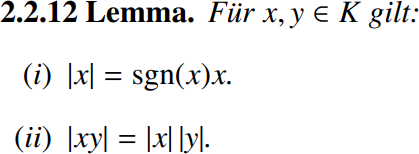
\includegraphics[width = 5 cm]{Kaltenbaeck - Fundament Analysis - Lemma 2-2-12-1.png} \\
      \vspace{0.01 cm}
      \hspace{0.5 cm}
      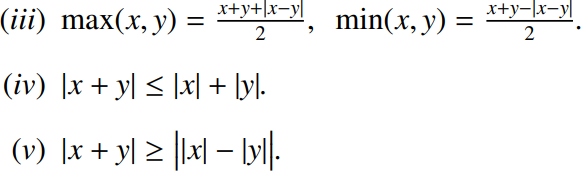
\includegraphics[width = 7 cm]{Kaltenbaeck - Fundament Analysis - Lemma 2-2-12-2.png} \\
      \vspace{0.5 cm}
      \caption{Kaltenbaeck - Fundament Analysis}
      \label{fig:KFAL2.2.12}
    \end{boxedin}
  \end{figure}

  \end{comment}

  Seien $c := 1/2$ und $d := 1$, dann gilt $\ForAlmostAll n \in \N:$

  \begin{multline*}
    c (f(n) + g(n))
    \leq
    \max \Bbraces{f(n), g(n)}
    =
    \frac{f(n) + g(n) + |f(n) - g(n)|}{2} \\
    \leq
    \frac{f(n) + g(n)}{2}
    +
    \frac{f(n) + g(n)}{2}
    =
    d (f(n) + g(n)).
  \end{multline*}

  \item Gegenbeispiel:
  Seien $f \equiv 0$ und $g \equiv 1$, dann gilt $\Forall c, d > 0:$

  \begin{align*}
    c \underbrace{(f(n) + g(n))}_1
    \not \leq
    \underbrace{\min \Bbraces{f(n), g(n)}}_0
    <
    d \underbrace{(f(n) + b(n))}_1.
  \end{align*}

  \begin{align*}
    \implies
    \min \Bbraces{f, g} \not \in \Theta(f + g)
  \end{align*}

  \item Gegenbeispiel:
  Seien $f(n) = n$ und $g(n) = -n$, für $n \in \N$, dann gilt wegen $|f| = |g|$ zwar $f \in \Landau(g)$, aber

  \begin{align*}
    \limsup_{n \to \infty}
    \vbraces
    {
      \frac
      {
        2^{f(n)}
      }{
        2^{g(n)}
      }
    }
    =
    \limsup_{n \to \infty}
    \vbraces
    {
      \frac
      {
        2^{n}
      }{
        2^{-n}
      }
    }
    =
    \limsup_{n \to \infty}
    2^{2n}
    =
    \infty
    \iff
    f \not \in \Landau(g).
  \end{align*}

  Gegenbeispiel:
  Seien $f = \log_2$ und $g = \log_4$, für $n \in \N$, dann gilt wegen $|f| = \log_2{4} |g|$ zwar $f \in \Landau(g)$, aber

  \begin{multline*}
    \limsup_{n  \to \infty}
    \vbraces
    {
      \frac
      {
        2^{f(n)}
      }{
        2^{g(n)}
      }
    }
    =
    \limsup_{n  \to \infty}
    \vbraces
    {
      \frac
      {
        2^{\log_2(n)}
      }{
        2^{\log_4(n)}
      }
    }
    =
    \limsup_{n  \to \infty}
    \vbraces
    {
      \frac
      {
        n
      }{
        2^\frac
        {
          \log_2(n)
        }{
          \log_2(4)
        }
      }
    }
    =
    \limsup_{n  \to \infty}
    \vbraces
    {
      \frac
      {
        n
      }{
        (2^{\log_2(n)})^{1/2}
      }
    } \\
    =
    \limsup_{n  \to \infty}
    \vbraces
    {
      \frac
      {
        n
      }{
        \sqrt{n}
      }
    }
    =
    \limsup_{n  \to \infty}
    \sqrt{n}
    =
    \infty
  \end{multline*}

  \item Gegenbeispiel:
  Sei $f(n) = 1/n$.

  \begin{align*}
    \implies
    \limsup_{n \to \infty}
    \vbraces
    {
      \frac{f(n)}{f(n)^2}
    }
    =
    \limsup_{n \to \infty}
    \vbraces
    {
      \frac{1/n)}{1/n^2}
    }
    =
    \limsup_{n \to \infty} |n|
    =
    \infty
    \iff
    f \not \in \Landau(f^2)
  \end{align*}

  \item Beispiel:

  \begin{align*}
    f(n)
    :=
    \begin{cases}
      0,   & n \in 2 \N, \\
      n^2, & n \in 2 \N - 1,
    \end{cases}
  \end{align*}

  \begin{align*}
    \implies
    \liminf_{n \to \infty}
    \vbraces
    {
      \frac{f(n)}{n}
    }
    & =
    \sup_{n \in \N}
    \inf_{k \geq n}
    \vbraces
    {
      \frac{f(k)}{k}
    }
    =
    0
    \iff
    f(n) \neq \Omega(n), \\
    \limsup_{n \to \infty}
    \vbraces
    {
      \frac{f(n)}{n}
    }
    & =
    \inf_{n \in \N}
    \sup_{k \geq n}
    \vbraces
    {
      \frac{f(k)}{k}
    }
    =
    \infty
    \iff
    f(n) \neq \Landau(n).
  \end{align*}

\end{enumerate}

\end{solution}

% --------------------------------------------------------------------------------


\printbibliography

\end{document}
